\section{실험 및 결과}
\label{sec:experiments}

실험은 앞 실험에서 확인된 한계를 다음 실험이 보완하는 순서로 진행한다. 먼저 추가 학습을 하지 않은 Alpamayo-R1이 가드 문장에 반응하는지 확인한다. 그다음 작은 VLM을 학습하여 가드와 행동의 관계 자체를 배울 수 있는지 살펴본다. 이 과정에서 단순한 정지/진행 문제는 장면만 보고도 답을 맞힐 수 있다는 한계가 드러난다. 이를 해결하기 위해 이후 실험에서는 같은 장면과 같은 행동 목표를 유지하고 가드만 바꾸어 정답이 달라지게 한다. 평가 범위도 정적 경계, 대기와 출발의 시간 조건, 정지와 차선 변경 순으로 넓힌다. 마지막 폐루프 실험에서는 학습된 가드만으로 충분한지, 실행 중에 별도 차단 장치가 필요한지를 살펴본다.

이 장에서 사용하는 "가드 준수 목표 완료"는 실험에서 제시한 가드를 지키면서 CoC의 행동 목표까지 끝냈다는 뜻이다. 실제 도로의 모든 위험이 제거되었다는 뜻은 아니다. 전체 실험의 질문과 대표 결과는 표~\ref{tab:suite}에 먼저 요약하였다.

\subsection{Alpamayo-R1 사전학습 상태 진단}

\paragraph{확인 목적.}
첫 실험의 질문은 간단하다. 학습하지 않은 가드 문장을 Alpamayo-R1의 CoC에 추가하면, 모델이 그 의미에 맞게 궤적을 바꾸는가? 이 실험은 차량 안전을 평가하지 않는다. 별도의 가드 학습 없이 문장만 추가해도 되는지를 먼저 확인하는 진단 실험이다.

\paragraph{비교 방법.}
장면과 기본 CoC는 그대로 두고 추가 문장만 바꾸었다. 하나는 기다리라는 가드이고, 다른 하나는 그와 반대로 진행을 허용하는 가드이다. 행동과 관계없는 문장도 비교에 사용하였다. 먼저 기본 CoC에 문장을 추가했을 때 2초 뒤 궤적이 얼마나 달라졌는지 계산하였다. 다음으로 서로 반대되는 두 가드가 만든 궤적의 차이를 계산하였다. 첫 번째 값은 모델이 추가 문장에 반응했는지를 보여준다. 두 번째 값은 단순히 문장이 들어온 것에 반응한 것이 아니라, 기다림과 진행이라는 반대 의미를 구별했는지를 보여준다.

\paragraph{결과.}
그림~\ref{fig:r1-diagnostic}에서 문장을 추가한 궤적은 기본 CoC의 궤적과 2초 뒤 0.263 m 차이가 났다. 즉, 모델은 추가 문장에 반응하였다. 그러나 기다리라는 가드와 진행을 허용하는 가드 사이의 차이는 0.008 m에 불과했다.

\paragraph{의미.}
이 결과는 Alpamayo-R1이 CoC에 문장이 추가된 사실에는 반응하지만, 서로 반대되는 가드의 의미에 맞추어 궤적을 바꾸지는 못했음을 뜻한다. 따라서 가드 문장을 넣는 것만으로 준수를 기대하기 어렵다. 다음 실험에서는 작은 VLM에 가드와 올바른 행동의 관계를 직접 학습시킨다.

\begin{figure}[t]
\centering
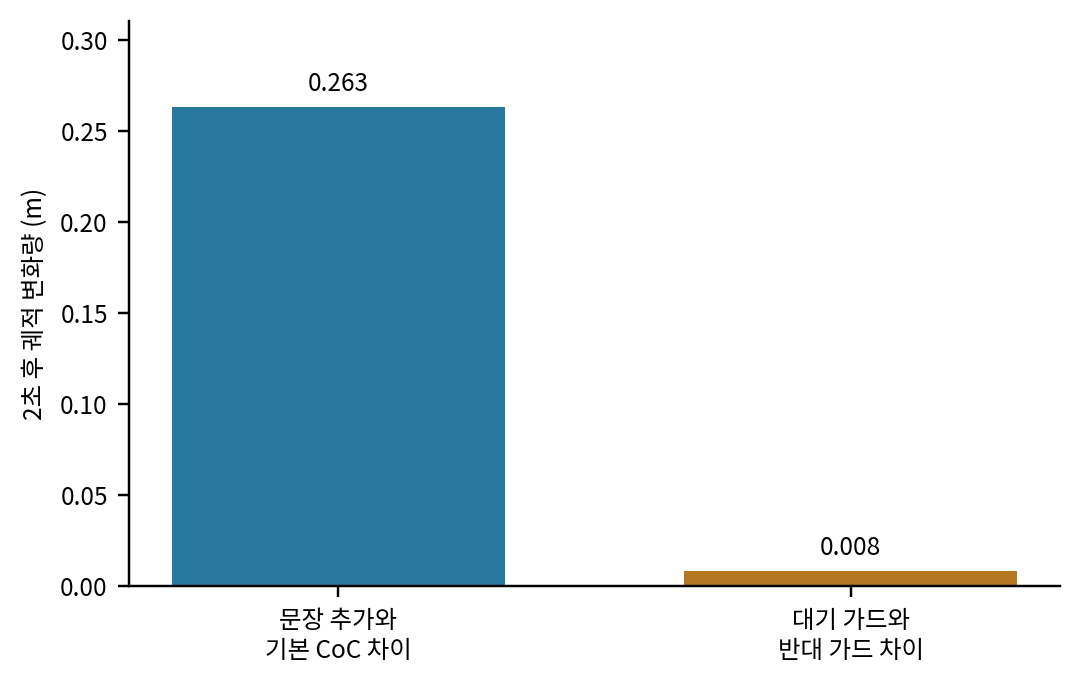
\includegraphics[width=0.94\columnwidth]{figures/fig04_r1_diagnostic.png}
\caption{Alpamayo-R1 사전 진단. 첫 막대는 문장을 추가했을 때 기본 CoC에서 궤적이 얼마나 달라졌는지를, 두 번째 막대는 서로 반대되는 두 가드 사이에서 궤적이 얼마나 달라졌는지를 나타낸다.}
\label{fig:r1-diagnostic}
\end{figure}

\subsection{최소 가드-행동 학습과 초기 과제의 한계}

\paragraph{확인 목적.}
두 번째 실험은 작은 VLM이 "이 가드에서는 정지하고, 저 가드에서는 진행한다"는 대응을 학습할 수 있는지 확인한다. 동시에 정지와 진행만 구분하는 쉬운 문제가 가드의 효과를 실제보다 크게 보이게 할 수 있는지도 확인한다.

\paragraph{비교 방법.}
후보는 정지(STOP)와 진행(PROCEED) 두 가지로 만들었다. 첫 조건에서는 가드와 정답 행동을 올바르게 연결했다. 비교 조건에서는 같은 가드 문장을 사용하되 정답 행동과의 연결을 일부러 섞었다. 이 비교를 통해 모델이 단순히 문장을 받은 효과와 가드의 올바른 의미를 배운 효과를 구분한다. 평가는 학습에 사용하지 않은 장면과, 같은 뜻을 다른 문장으로 표현한 경우로 나누었다. 쉬운 과제에서는 학습량의 차이가 결과에 영향을 주지 않도록 기존 CoC와 CoC+Guard의 학습 횟수도 같게 맞추었다.

\paragraph{결과.}
학습에 사용하지 않은 장면에서 올바른 가드 대응 조건의 정확도는 0.990, 쌍 정확도는 0.958이었다. 반면 대응을 섞은 조건은 각각 0.719와 0.000이었다. 이는 올바른 가드--행동 관계를 학습하면 새로운 장면에서도 두 가드를 구별할 수 있음을 보여준다. 그러나 같은 뜻을 다른 문장으로 바꾼 평가에서는 두 조건의 정확도가 0.740과 0.745였고, 쌍 정확도는 모두 0이었다. 즉, 학습한 문장과 비슷한 표현에는 잘 대응했지만 새로운 표현까지 이해하지는 못했다.

또한 학습 자료가 충분한 쉬운 과제에서는 기존 CoC만 사용해도 정확도 0.974와 쌍 정확도 0.896에 도달했고, CoC+Guard는 1.000과 1.000이었다. 학습 횟수를 같게 맞춘 사후 비교에서는 두 조건 모두 1.000이었다.

\paragraph{의미.}
두 가지를 알 수 있다. 첫째, 작은 VLM은 가드와 행동의 관계를 학습할 수 있다. 둘째, 쉬운 정지/진행 문제에서는 가드가 없어도 장면만 보고 정답을 외울 수 있다. 이 경우 CoC+Guard의 높은 정확도가 정말 가드를 읽은 결과인지 분명하지 않다. 따라서 다음 실험부터는 모든 후보가 같은 CoC 목표를 달성하게 만들고, 가드를 지키는지와 얼마나 원활하게 진행하는지만 다르게 구성한다.

\begin{table*}[!t]
\centering
\caption{주요 실험의 비교 대상, 대표 결과 및 의미.}
\label{tab:suite}
\scriptsize
\begin{tabularx}{\textwidth}{L{0.14\textwidth}L{0.19\textwidth}L{0.20\textwidth}L{0.20\textwidth}Y}
\toprule
실험 & 주요 비교 & 핵심 측정값 & 대표 결과 & 의미 \\
\midrule
R1 사전 진단 & 기본 CoC, 대기 가드, 반대 가드 & 2초 후 궤적 변화량 & 기본 CoC와 0.263 m 차이, 반대 가드끼리는 0.008 m 차이 & 문장에는 반응하지만 반대 의미를 구별하지 못함 \\
최소 학습 & 올바른 가드 대응, 대응을 섞은 가드 & 새 장면 정확도, 쌍 정확도 & 올바른 대응 0.990/0.958, 섞은 대응 0.719/0.000 & 가드-행동 관계는 배우지만 새로운 표현에는 약함 \\
정적 후보 & 요구사항 전용형과 네 가드 표현 & 위반률, 보수 선택률, 쌍 정확도 & CoC 통합형: 위반 0.000, 쌍 정확도 1.000 & 같은 목표의 후보 중 가드에 맞는 선택이 가능 \\
시간 조건 & 대기시간이 다른 두 계약 & 가드 위반, 목표 완료, 쌍 정확도 & 요구사항 전용형 위반 0.319, CoC 통합형 0.000 & 대기와 해제 조건을 학습해 선택을 바꿀 수 있음 \\
다중 주행 & 정지, 차선 변경, 어려운 표현 & 위반률, 목표 완료, 쌍 정확도 & 일반 평가 위반 0.000, 어려운 표현 평가 0.010 & 효과가 여러 행동으로 확장되지만 단위 변환 오류가 남음 \\
폐루프 보조 & 상태, CoC, 상황에 따라 바뀌는 계약, 차단장치 & 가드 위반, 충돌, 개입 횟수 & 재위험 상황 위반 46.6\%에서 21.4\%, 차단장치 사용 시 4.8\% & 학습된 계약만으로 부족하며 최신 상태를 이용한 실행 검사가 필요 \\
\bottomrule
\end{tabularx}
\end{table*}

\subsection{동일 목표를 달성하는 정적 궤적 후보}

\paragraph{확인 목적.}
이 실험에서는 모든 후보가 "교차로를 통과한다"는 같은 목표를 달성한다. 따라서 모델은 목표 달성 여부만으로 정답을 고를 수 없다. 현재 가드가 어느 후보를 허용하는지 읽어야 한다.

\paragraph{비교 방법.}
두 후보 모두 교차로를 통과하지만 최대 속도, 장애물과의 최소거리, 진입 시점과 진행 속도가 다르다. 같은 장면에서 완화 계약은 더 빠른 후보를 허용하지만, 엄격 계약은 그 후보를 금지하고 더 신중한 후보를 허용한다. 요구사항 전용형, CoC 통합형, 가드 분리형, 대응을 섞은 가드와 논리식 가드를 비교하였다. 두 계약의 정답을 모두 맞혀야 하는 쌍 정확도를 핵심 지표로 사용하였다.

\begin{table*}[!t]
\centering
\caption{같은 CoC 목표를 달성하는 정적 후보의 분리 평가 결과.}
\label{tab:static}
\footnotesize
\begin{tabular}{lccccc}
\toprule
조건 & 후보 정확도 & 가드 위반 $\downarrow$ & 과도한 보수 $\downarrow$ & 쌍 정확도 $\uparrow$ & 목표 완료 \\
\midrule
요구사항 전용형 & 0.500 & 0.500 & 0.500 & 0.000 & 1.000 \\
CoC 통합형 & \textbf{1.000} & \textbf{0.000} & \textbf{0.000} & \textbf{1.000} & 1.000 \\
가드 분리형 & 0.993 & 0.014 & 0.000 & 0.986 & 1.000 \\
대응을 섞은 가드 & 0.465 & 0.375 & 0.694 & 0.153 & 1.000 \\
논리식 가드 & \textbf{1.000} & \textbf{0.000} & \textbf{0.000} & \textbf{1.000} & 1.000 \\
\bottomrule
\end{tabular}
\end{table*}

\paragraph{결과.}
표~\ref{tab:static}에서 모든 조건의 목표 완료율은 1.000이었다. 즉, 어느 조건도 교차로 통과 자체를 포기하지 않았다. 그러나 가드가 없는 요구사항 전용형은 선택의 절반에서 가드를 위반하여 위반률이 0.500이었고, 두 계약을 모두 맞힌 쌍은 없어 쌍 정확도가 0.000이었다. 대응을 섞은 조건의 쌍 정확도도 0.153에 머물렀다.

반면 CoC 통합형과 논리식 가드는 위반률 0.000, 과도한 보수 선택률 0.000, 쌍 정확도 1.000을 기록하였다. 가드 분리형도 위반률 0.014와 쌍 정확도 0.986으로 높았다. 이 조건들은 같은 장면에서도 계약이 바뀌면 정답 후보를 함께 바꾸었다.

문장을 바꾸어 쓴 평가의 정확도와 쌍 정확도는 CoC 통합형 0.875/0.750, 가드 분리형 0.924/0.847, 논리식 가드 1.000/1.000이었다. 학습하지 않은 수치를 사용한 평가는 각각 1.000/1.000, 0.951/0.903, 0.924/0.847이었다.

\paragraph{의미.}
CoC 통합형은 항상 정지하는 방법으로 위반을 피한 것이 아니다. 모든 후보가 목표를 완료했고, 그중 현재 계약이 허용하는 가장 원활한 후보를 골랐다. 따라서 이 결과는 모델이 실행 가드를 후보 선택에 사용했음을 보여준다. 다만 정적 과제에서 논리식 가드가 높은 성능을 보였다는 이유만으로 논리 표현이 언제나 더 좋다고 결론 내릴 수는 없다. 다음 시간 과제에서는 다른 결과가 나타난다.

\subsection{정지-대기-해제-출발 시간 조건}

\paragraph{확인 목적.}
앞 실험은 속도나 거리처럼 한 시점의 기준을 다루었다. 이번 실험은 "얼마나 오래 기다려야 하며 언제 출발해도 되는가"라는 시간 조건도 모델이 배울 수 있는지 확인한다.

\paragraph{비교 방법.}
장면과 네 후보는 그대로 두고, 상충 구역이 비어 있는 것을 확인한 뒤 기다려야 하는 시간만 바꾸었다. 완화 계약은 짧게 기다린 뒤 출발하는 후보를 허용하고, 엄격 계약은 더 오래 기다린 후보만 허용한다. 후보는 조기 진입, 짧은 대기 후 진입, 긴 대기 후 진입과 계속 정지로 구성하였다. 결과가 학습의 무작위성에 좌우되는지 확인하기 위해 요구사항 전용형과 네 가지 가드 표현을 서로 다른 초기값 42, 17, 123으로 각각 학습하였다.

\begin{table*}[!t]
\centering
\caption{정지-대기-해제-출발 시간 조건의 3회 반복 평균과 표준편차.}
\label{tab:temporal}
\footnotesize
\begin{tabular}{lccccc}
\toprule
조건 & 후보 정확도 & 가드 위반 $\downarrow$ & 교착 $\downarrow$ & 가드 준수 목표 완료 $\uparrow$ & 쌍 정확도 $\uparrow$ \\
\midrule
요구사항 전용형 & $0.500\pm0.000$ & $0.319\pm0.052$ & $0.000\pm0.000$ & $0.681\pm0.052$ & $0.000\pm0.000$ \\
CoC 통합형 & $\mathbf{1.000\pm0.000}$ & $\mathbf{0.000\pm0.000}$ & $0.000\pm0.000$ & $\mathbf{1.000\pm0.000}$ & $\mathbf{1.000\pm0.000}$ \\
가드 분리형 & $0.698\pm0.094$ & $0.191\pm0.136$ & $0.000\pm0.000$ & $0.809\pm0.136$ & $0.396\pm0.187$ \\
대응을 섞은 가드 & $0.510\pm0.015$ & $0.333\pm0.023$ & $0.000\pm0.000$ & $0.667\pm0.023$ & $0.021\pm0.029$ \\
논리식 가드 & $0.538\pm0.027$ & $0.274\pm0.108$ & $0.000\pm0.000$ & $0.726\pm0.108$ & $0.076\pm0.055$ \\
\bottomrule
\end{tabular}
\end{table*}

\paragraph{결과.}
표~\ref{tab:temporal}과 그림~\ref{fig:temporal-pair}(a)에서 CoC 통합형은 세 번의 반복 모두 가드 위반 0.000, 가드 준수 목표 완료 1.000, 쌍 정확도 1.000을 기록하였다. 대기시간이 바뀔 때마다 짧은 대기 후보와 긴 대기 후보를 올바르게 바꾼 것이다. 반면 요구사항 전용형의 가드 위반률은 $0.319\pm0.052$였고 쌍 정확도는 0이었다. 가드 분리형은 평균적으로 요구사항 전용형보다 나았지만 초기값에 따라 결과 차이가 컸다. 대응을 섞은 가드와 논리식 가드는 두 대기시간의 차이를 안정적으로 배우지 못했다.

\paragraph{의미.}
CoC 통합형은 단순히 정지와 진행을 구별한 것이 아니다. 같은 장면에서도 가드가 요구하는 대기시간을 읽고 출발 시점을 바꾸었다. 한편 논리식 가드의 낮은 결과는 논리식 자체가 자연어보다 나쁘다는 뜻이 아니다. 기반 VLM이 자연어에는 익숙하지만 현재 사용한 논리 문법에는 충분히 적응하지 못했을 수 있다. 두 표현을 공정하게 비교하려면 논리 문법을 따로 학습시킨 뒤 다시 평가해야 한다.

\subsection{정지·차선 변경과 어려운 표현}

\paragraph{확인 목적.}
앞 실험의 성공이 대기시간 문제에만 나타난 결과일 수 있다. 이를 확인하기 위해 정지와 차선 변경으로 행동을 넓혔다. 또한 같은 가드를 다른 문장이나 처음 보는 수치로 표현해도 모델이 조건을 지키는지 확인하였다.

\paragraph{비교 방법.}
정지 과제에서는 정지선 위치, 최대 감속도와 최대 가가속도를 가드로 사용하였다. 차선 변경 과제에서는 최소 차량 간격과 중단 후 재시도 조건을 사용하였다. 192개 장면마다 완화 계약과 엄격 계약을 하나씩 적용하여 384개 학습 예를 만들었다. 일반 평가, 같은 뜻을 바꾸어 쓴 문장 평가와 학습하지 않은 수치 평가는 각각 48개 장면, 즉 96개 계약 문제로 구성하였다. 별도의 어려운 표현 평가에는 기준값과 정확히 같은 경우, 부정·금지 문장, 조건문의 순서 변경과 m를 cm로 바꾼 문장을 함께 넣었다.

\begin{table*}[!t]
\centering
\caption{다중 주행 과제의 일반 평가와 어려운 표현 평가 결과. 값은 3회 반복 평균과 표준편차다.}
\label{tab:maneuver}
\footnotesize
\begin{tabular}{llcccc}
\toprule
평가 & 조건 & 후보 정확도 & 가드 위반 $\downarrow$ & 가드 준수 목표 완료 $\uparrow$ & 쌍 정확도 $\uparrow$ \\
\midrule
일반 & 요구사항 전용형 & $0.500\pm0.000$ & $0.292\pm0.072$ & $0.708\pm0.072$ & $0.000\pm0.000$ \\
 & Safety-Constrained CoC & $\mathbf{1.000\pm0.000}$ & $\mathbf{0.000\pm0.000}$ & $\mathbf{1.000\pm0.000}$ & $\mathbf{1.000\pm0.000}$ \\
 & 대응을 섞은 가드 & $0.503\pm0.006$ & $0.267\pm0.039$ & $0.733\pm0.039$ & $0.028\pm0.032$ \\
\midrule
어려운 표현 & 요구사항 전용형 & $0.500\pm0.000$ & $0.302\pm0.065$ & $0.698\pm0.065$ & $0.000\pm0.000$ \\
 & Safety-Constrained CoC & $\mathbf{0.948\pm0.063}$ & $\mathbf{0.010\pm0.010}$ & $\mathbf{0.990\pm0.010}$ & $\mathbf{0.896\pm0.127}$ \\
 & 대응을 섞은 가드 & $0.535\pm0.079$ & $0.260\pm0.018$ & $0.740\pm0.018$ & $0.090\pm0.139$ \\
\bottomrule
\end{tabular}
\end{table*}

\paragraph{결과.}
일반 평가에서 Safety-Constrained CoC는 정지와 차선 변경 모두 가드 위반 0.000, 가드 준수 목표 완료 1.000, 쌍 정확도 1.000을 기록하였다. 즉, 두 행동에서 목표를 완료하면서 완화·엄격 계약의 정답을 모두 바꾸어 골랐다. 요구사항 전용형보다 평균 위반률은 0.292 낮았다. 초기값을 단위로 다시 뽑아 계산한 95\% 구간은 [0.250, 0.375]였다. 대응을 섞은 가드보다 쌍 정확도는 0.972 높았고 해당 구간은 [0.938, 1.000]이었다. 다만 학습을 세 번만 반복했으므로 이 구간은 확정적인 통계 결론이 아니라 결과의 범위를 살펴보는 참고값이다.

어려운 표현 평가에서는 가드 위반률이 $0.010\pm0.010$, 쌍 정확도가 $0.896\pm0.127$로 낮아졌다. 오답 15개는 모두 같은 거리를 m 대신 cm로 표현한 문장에서 발생하였다. 초기값 42에서 나온 오답 12개는 가드를 어기지는 않았지만 필요 이상으로 느린 차선 변경 후보를 선택한 경우였다. 나머지 3개는 감속도 또는 가가속도 상한을 넘은 정지 후보를 선택한 경우였다. 부정 표현, 조건문의 순서 변경과 m 단위 경계값만 포함한 예에서는 오답이 없었다.

\paragraph{의미.}
가드를 CoC 안에 함께 제시하는 효과는 대기시간뿐 아니라 정지와 차선 변경에서도 나타났다. 그러나 단위를 바꾼 문장에서는 오류가 남았다. 이번 어려운 표현 평가에는 여러 변화가 함께 포함되었으므로, 모든 오류의 원인이 단위 변환이라고 확정할 수는 없다. 후속 실험에서는 단위, 부정 표현, 조건 순서와 경계값을 한 번에 하나씩만 바꾸어 원인을 분리해야 한다.

\begin{figure*}[!t]
\centering
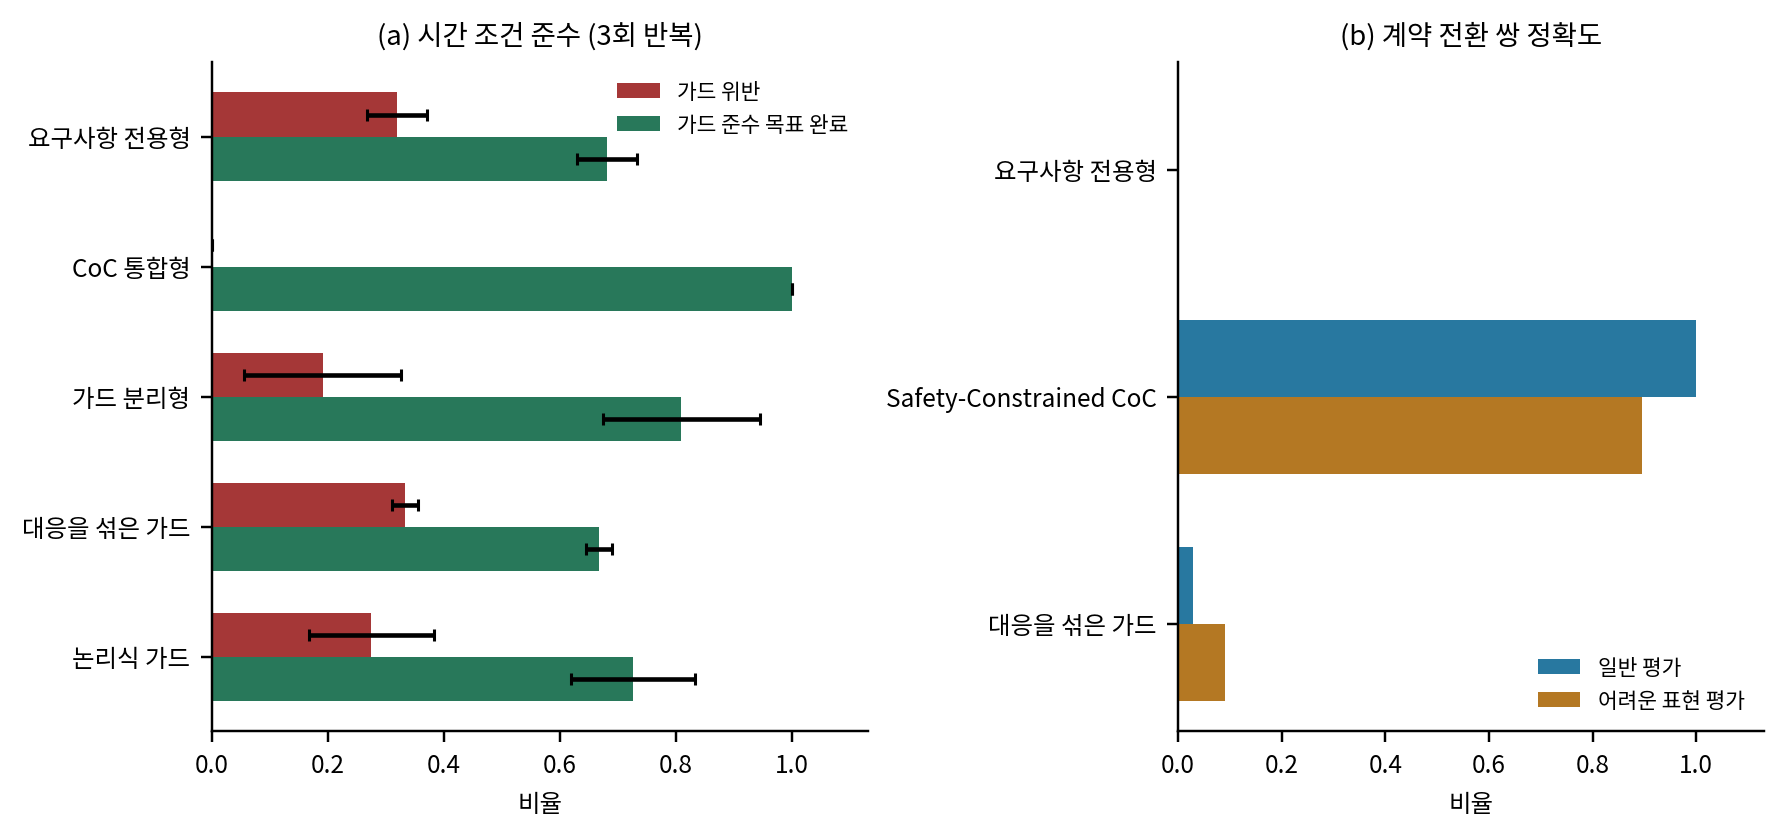
\includegraphics[width=0.98\textwidth]{figures/fig05_temporal_pair.png}
\caption{시간 조건과 다중 주행 과제의 결과. (a)는 시간 조건별 가드 위반률과 가드 준수 목표 완료율, (b)는 일반 평가와 어려운 표현 평가의 계약 전환 쌍 정확도를 비교한다. 오차 막대는 3회 반복의 표준편차다.}
\label{fig:temporal-pair}
\end{figure*}

\subsection{폐루프 보조 실험}

\paragraph{확인 목적.}
앞의 실험은 VLM이 미리 주어진 후보를 한 번 선택하는 문제였다. 마지막 실험은 선택 뒤에도 상황이 계속 바뀌는 경우를 살펴본다. 학습된 계약만 사용할 때와, 실행 중 위험한 명령을 막는 차단 장치를 함께 사용할 때를 비교한다. 이 실험은 작은 신경망과 단순한 운동 모델을 사용한 보조 분석이며, 앞의 VLM 결과나 실제 차량과 직접 비교하지 않는다.

\paragraph{비교 방법.}
두 층 신경망과 1차원 운동학으로 만든 소규모 폐루프 환경을 사용하였다. 폐루프란 모델이 한 번만 답하는 것이 아니라, 매 시점의 상태를 다시 받아 다음 행동을 계속 정하는 환경을 뜻한다. 상태만 주는 조건, 상태와 CoC를 주는 조건, 상황에 따라 바뀌는 동적 계약, 한 번 진행으로 바뀌면 다시 대기로 돌아가지 않는 단조 단계 계약과 계약+차단장치를 비교하였다.

평가는 두 상황으로 나누었다. 첫째, 학습 자료에 정지, 대기, 출발 등 모든 주행 단계가 충분히 들어 있는 상황이다. 둘째, 출발이 허용된 뒤 다른 차량이 다시 나타나므로 다시 정지해야 하지만 학습에서는 보지 못한 "해제 후 위험 재등장" 상황이다. 앞으로 1.2초의 모든 상황을 미리 아는 조건도 넣었지만, 이는 실제 방법이 아니라 도달 가능한 가장 좋은 결과를 보기 위한 참고값이다.

\begin{figure*}[!t]
\centering
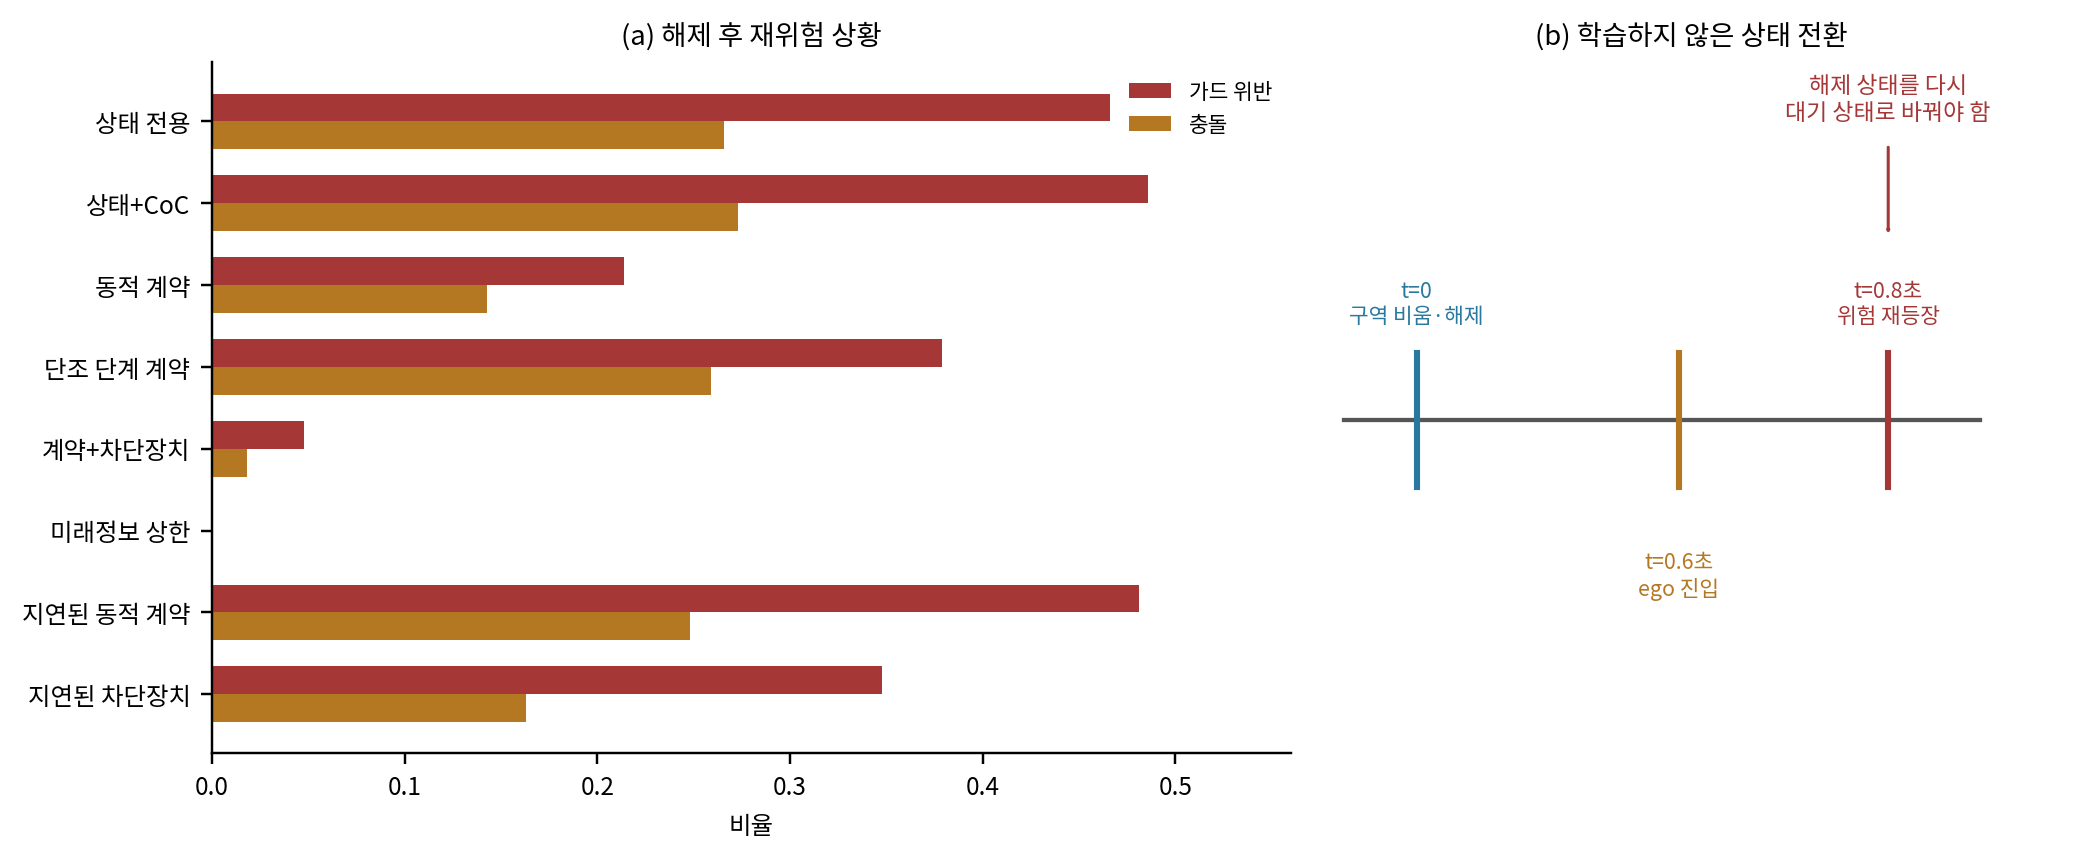
\includegraphics[width=0.98\textwidth]{figures/fig06_release_reversal.png}
\caption{폐루프 보조 실험. (a)는 출발이 허용된 뒤 위험이 다시 나타나는 상황에서 각 방법의 가드 위반률과 충돌률을 비교한다. (b)는 출발 허용, 다른 차량의 진입, 다시 정지해야 하는 순간의 순서를 보여준다. 미래정보 상한은 앞으로의 상황을 완벽히 안다고 가정한 참고값이며 실제 적용 방법이 아니다.}
\label{fig:release-reversal}
\end{figure*}

\paragraph{결과.}
먼저 모든 주행 단계를 학습한 상황을 보았다. 정지 후 대기로 넘어가는 예 1,404개를 학습 자료에 추가하자 상태 전용, 상태+CoC, 동적 계약과 단조 단계 계약 모두 300회 평가에서 정지 구간에 너무 일찍 들어가지 않았다. 학습 분포 밖 상황의 가드 위반률도 상태 전용 2.6\%, 상태+CoC 1.4\%, 동적 계약, 단조 단계 계약과 계약+차단장치는 모두 0\%였다. 이 경우 차단장치는 위반률을 더 낮추지 못했지만 주행할 때마다 평균 2.539회 개입했다. 이미 학습으로 해결된 상황에서는 차단장치가 불필요하게 작동할 수 있음을 뜻한다.

그러나 그림~\ref{fig:release-reversal}의 해제 후 재위험 상황에서는 결과가 달랐다. 가드 위반률은 상태 전용 46.6\%, 상태+CoC 48.6\%, 동적 계약 21.4\%, 단조 단계 계약 37.9\%, 계약+차단장치 4.8\%였다. 동적 계약은 현재 위험 상태를 알려 주어 위반을 줄였고, 차단장치는 위험한 행동을 실행 직전에 막아 위반을 더 줄였다. 충돌률도 같은 순서로 26.6\%, 27.3\%, 14.3\%, 25.9\%, 1.8\%였다.

모든 조건의 목표 완료율은 100\%였으므로 낮은 위반률이 단순히 차량을 계속 세운 결과는 아니었다. 앞으로의 상황을 완벽히 아는 비현실적 조건만 위반과 충돌이 모두 0\%였다. 또한 계약 정보가 실제 상황보다 0.4초 늦게 도착하면 동적 계약의 위반률은 48.1\%, 계약+차단장치는 34.8\%로 증가하였다. 올바른 계약도 늦게 전달되면 효과가 크게 줄어든다는 뜻이다.

\paragraph{의미.}
충분한 성공 시연이 있으면 모델은 문장에 적히지 않은 일부 제약도 행동 예에서 배울 수 있다. 이때 차단장치를 항상 사용하면 성능을 더 높이지 못하면서 개입만 늘어날 수 있다. 그러나 학습하지 않은 위험이 다시 나타나면 동적 계약만으로는 위반을 모두 막지 못했다. 최신 상태를 사용하는 차단장치를 함께 사용했을 때 위반과 충돌이 가장 크게 줄었다. 그 효과도 계약 정보가 늦으면 감소했다. 따라서 학습된 가드는 도움이 되지만, 새로운 위험과 정보 지연까지 혼자서 해결하지는 못한다.
